%%%%%%%%%%%%%%%%%%%%%%%%%%%%%%%%%%%%%%%%%
% Beamer Presentation
% LaTeX Template
% Version 2.0 (March 8, 2022)
%
% This template originates from:
% https://www.LaTeXTemplates.com
%
% Author:
% Vel (vel@latextemplates.com)
%
% License:
% CC BY-NC-SA 4.0 (https://creativecommons.org/licenses/by-nc-sa/4.0/)
%
%%%%%%%%%%%%%%%%%%%%%%%%%%%%%%%%%%%%%%%%%

%----------------------------------------------------------------------------------------
%	PACKAGES AND OTHER DOCUMENT CONFIGURATIONS
%----------------------------------------------------------------------------------------
\documentclass[
	11pt, % Set the default font size, options include: 8pt, 9pt, 10pt, 11pt, 12pt, 14pt, 17pt, 20pt
	%t, % Uncomment to vertically align all slide content to the top of the slide, rather than the default centered
	%aspectratio=169, % Uncomment to set the aspect ratio to a 16:9 ratio which matches the aspect ratio of 1080p and 4K screens and projectors
]{beamer}

\graphicspath{{Images/}{./}} % Specifies where to look for included images (trailing slash required)

\usepackage{booktabs} % Allows the use of \toprule, \midrule and \bottomrule for better rules in tables

%----------------------------------------------------------------------------------------
%	SELECT LAYOUT THEME
%----------------------------------------------------------------------------------------

% Beamer comes with a number of default layout themes which change the colors and layouts of slides. Below is a list of all themes available, uncomment each in turn to see what they look like.

%\usetheme{default}
%\usetheme{AnnArbor}
%\usetheme{Antibes}
%\usetheme{Bergen}
%\usetheme{Berkeley}
%\usetheme{Berlin}
\usetheme{Boadilla} %me gusta
%\usetheme{CambridgeUS}
%\usetheme{Copenhagen}
%\usetheme{Darmstadt}
%\usetheme{Dresden}
%\usetheme{Frankfurt}
%\usetheme{Goettingen} %dos dos
%\usetheme{Hannover} %dos dos
%\usetheme{Ilmenau}
%\usetheme{JuanLesPins}
%\usetheme{Luebeck}
%\usetheme{Madrid}
%\usetheme{Malmoe}
%\usetheme{Marburg}
%\usetheme{Montpellier}
%\usetheme{PaloAlto}
%\usetheme{Pittsburgh}
%\usetheme{Rochester} %muy flat
%\usetheme{Singapore}
%\usetheme{Szeged}
%\usetheme{Warsaw}

%----------------------------------------------------------------------------------------
%	SELECT COLOR THEME
%----------------------------------------------------------------------------------------

% Beamer comes with a number of color themes that can be applied to any layout theme to change its colors. Uncomment each of these in turn to see how they change the colors of your selected layout theme.

%\usecolortheme{albatross}
%\usecolortheme{beaver}
%\usecolortheme{beetle}
%\usecolortheme{crane}
%\usecolortheme{dolphin}
%\usecolortheme{dove}
%\usecolortheme{fly}
%\usecolortheme{lily} %default
%\usecolortheme{monarca}
%\usecolortheme{seagull}
%\usecolortheme{seahorse}
%\usecolortheme{spruce}
%\usecolortheme{whale}
%\usecolortheme{wolverine}

%----------------------------------------------------------------------------------------
%	SELECT FONT THEME & FONTS
%----------------------------------------------------------------------------------------

% Beamer comes with several font themes to easily change the fonts used in various parts of the presentation. Review the comments beside each one to decide if you would like to use it. Note that additional options can be specified for several of these font themes, consult the beamer documentation for more information.

\usefonttheme{default} % Typeset using the default sans serif font
%\usefonttheme{serif} % Typeset using the default serif font (make sure a sans font isn't being set as the default font if you use this option!)
%\usefonttheme{structurebold} % Typeset important structure text (titles, headlines, footlines, sidebar, etc) in bold
%\usefonttheme{structureitalicserif} % Typeset important structure text (titles, headlines, footlines, sidebar, etc) in italic serif
%\usefonttheme{structuresmallcapsserif} % Typeset important structure text (titles, headlines, footlines, sidebar, etc) in small caps serif

%------------------------------------------------

%\usepackage{mathptmx} % Use the Times font for serif text
\usepackage{palatino} % Use the Palatino font for serif text

\usepackage[ruled,vlined]{algorithm2e}
%\usepackage{helvet} % Use the Helvetica font for sans serif text
\usepackage[default]{opensans} % Use the Open Sans font for sans serif text
\usepackage[spanish]{babel}
\usepackage{dirtree}
\usepackage{xcolor}
%\usepackage[default]{FiraSans} % Use the Fira Sans font for sans serif text
%\usepackage[default]{lato} % Use the Lato font for sans serif text

\usepackage[scaled]{helvet}
\usepackage[round]{natbib}
%\newcommand{\newblock}{}

\usepackage{rotating}

\newcommand\FourQuad[4]{%
  \begin{minipage}[b][.33\textheight][t] 
    {.48\textwidth}#1\end{minipage}\hfill%
    \begin{minipage}[b][.33\textheight][t] 
      {.48\textwidth}#2\end{minipage}\\[0.5em]
      \begin{minipage}[b][.33\textheight][t] 
        {.48\textwidth}#3\end{minipage}\hfill
        \begin{minipage}[b][.33\textheight][t] 
          {.48\textwidth}#4\end{minipage}%
}

\usepackage{tikz}
\usetikzlibrary{arrows,shapes,positioning,shadows,trees,quotes}

\tikzset{
  basic/.style  = {draw, text width=2cm, drop shadow, font=\sffamily, rectangle},
  root/.style   = {basic, rounded corners=2pt, thin, align=center,
                   fill=green!30},
  level 2/.style = {basic, rounded corners=6pt, thin,align=center, fill=green!60,
                   text width=8em},
  level 3/.style = {basic, thin, align=left, fill=pink!60, text width=6.5em}
}

\usepackage{array} % needed for \arraybackslash
\usepackage{graphicx}
\usepackage{adjustbox} % for \adjincludegraphics

\usepackage{subcaption}
\usepackage{bibentry}
%\bibliographystyle{apalike}
\usepackage{chngcntr}
\usepackage{lipsum}% http://ctan.org/pkg/lipsum
\usepackage{hanging}% http://ctan.org/pkg/hanging

%----------------------------------------------------------------------------------------
%	SELECT INNER THEME
%----------------------------------------------------------------------------------------

% Inner themes change the styling of internal slide elements, for example: bullet points, blocks, bibliography entries, title pages, theorems, etc. Uncomment each theme in turn to see what changes it makes to your presentation.

%\useinnertheme{default}
\useinnertheme{circles}
%\useinnertheme{rectangles}
%\useinnertheme{rounded}
%\useinnertheme{inmargin}

%----------------------------------------------------------------------------------------
%	SELECT OUTER THEME
%----------------------------------------------------------------------------------------

% Outer themes change the overall layout of slides, such as: header and footer lines, sidebars and slide titles. Uncomment each theme in turn to see what changes it makes to your presentation.

%\useoutertheme{default}
%\useoutertheme{infolines}
%\useoutertheme{miniframes}
%\useoutertheme{smoothbars}
%\useoutertheme{sidebar}
%\useoutertheme{split}
%\useoutertheme{shadow}
%\useoutertheme{tree}
%\useoutertheme{smoothtree}

%\setbeamertemplate{footline} % Uncomment this line to remove the footer line in all slides
%\setbeamertemplate{footline}[page number] % Uncomment this line to replace the footer line in all slides with a simple slide count
\setbeamertemplate{caption}[numbered]
%\setbeamertemplate{navigation symbols}{} % Uncomment this line to remove the navigation symbols from the bottom of all slides

%----------------------------------------------------------------------------------------
%	PRESENTATION INFORMATION
%----------------------------------------------------------------------------------------

\title[SEMINARIO DE INVESTIGACIÓN I]{%\centering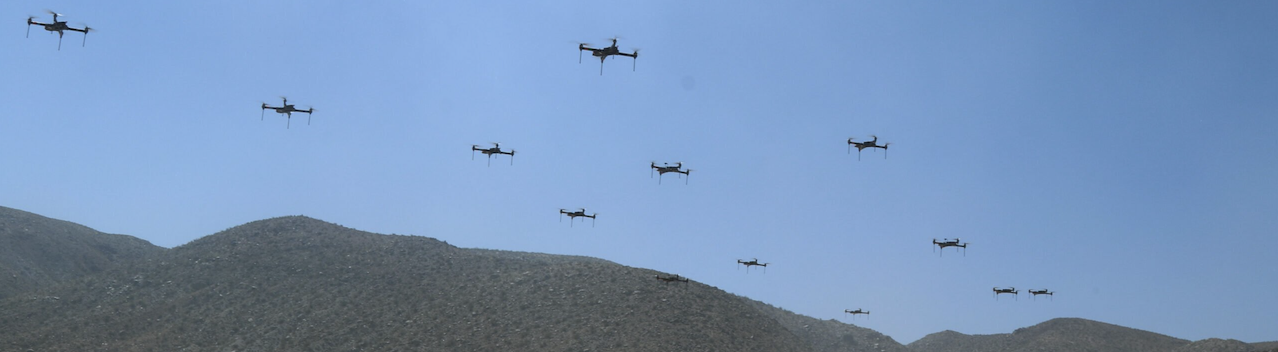
\includegraphics[width=10cm]{swarm_drones}\\
  Estrategias para la exploración coordinada multi-VANT} % The short title in the optional parameter appears at the bottom of every slide, the full title in the main parameter is only on the title page

%\subtitle{Optional Subtitle} % Presentation subtitle, remove this command if a subtitle isn't required

\author[Luis Ballado]{Luis Alberto Ballado Aradias} % Presenter name(s), the optional parameter can contain a shortened version to appear on the bottom of every slide, while the main parameter will appear on the title slide

\institute[CINVESTAV]{
  CINVESTAV UNIDAD TAMAULIPAS \\
  %\smallskip \textit{luis.ballado@cinvestav.mx}
} % Your institution, the optional parameter can be used for the institution shorthand and will appear on the bottom of every slide after author names, while the required parameter is used on the title slide and can include your email address or additional information on separate lines

\date[\today]{Cd. Victoria, Tamaulipas - \today} % Presentation date or conference/meeting name, the optional parameter can contain a shortened version to appear on the bottom of every slide, while the required parameter value is output to the title slide

%\titlegraphic{\hspace*{8.75cm}~%
%   
\includegraphics[width=0.8cm]{cinvestavlogo}
%}

%----------------------------------------------------------------------------------------

\counterwithin*{footnote}{page}
\newcommand\footcite[1]{\footnote{\bibentry{#1}}\label{\thepage:#1}}
\newcommand\secondcite[1]{\textsuperscript{\ref{\thepage:#1}}}

\begin{document}

%----------------------------------------------------------------------------------------
%	TITLE SLIDE
%----------------------------------------------------------------------------------------

\begin{frame}
  \titlepage % Output the title slide, automatically created using the text entered in the PRESENTATION INFORMATION block above
\end{frame}

%----------------------------------------------------------------------------------------
%	TABLE OF CONTENTS SLIDE
%----------------------------------------------------------------------------------------

% The table of contents outputs the sections and subsections that appear in your presentation, specified with the standard \section and \subsection commands. You may either display all sections and subsections on one slide with \tableofcontents, or display each section at a time on subsequent slides with \tableofcontents[pausesections]. The latter is useful if you want to step through each section and mention what you will discuss.
\AtBeginSection[]
{
  \begin{frame}
    \frametitle{Contenido} % Slide title, remove this command for no title
    \tableofcontents[currentsection] % Output the table of contents (all sections on one slide)
    %\tableofcontents[pausesections] % Output the table of contents (break sections up across separate slides)
  \end{frame}
}
%----------------------------------------------------------------------------------------
%	PRESENTATION BODY SLIDES
%----------------------------------------------------------------------------------------

%\section{Introducción} % Sections are added in order to organize your presentation into discrete blocks, all sections and subsections are automatically output to the table of contents as an overview of the talk but NOT output in the presentation as separate slides

%------------------------------------------------

% Ejemplo imagen
%\begin{figure}
%  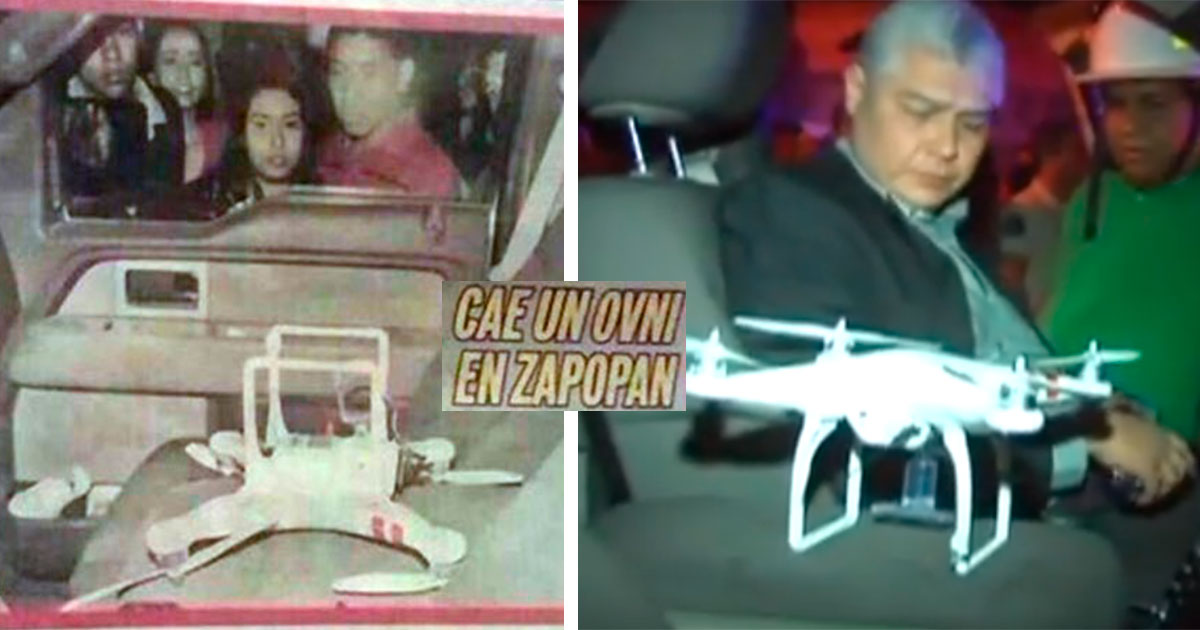
\includegraphics[width=0.7\linewidth]{dron_ovni.jpg}
%\end{figure}

\section{Resumen}

\begin{frame}{Robots A\'{e}reos}
  Actualmente vemos VANTS o coloquialmente como drones, a los que se le pueden pasar rutas de puntos GPS para que recorra, pero no est\'{a} siendo aut\'{o}nomo, sólo el piloto es reemplazado por un piloto autom\'{a}tico.\\
  \bigskip % Vertical whitespace
  \begin{itemize}
  \item Ala fija (tipo avi\'{o}n)
  \item Ala rotatoria coaxial (tipo helic\'{o}ptero)
  \item Alas rotatorias no coaxiales
  \end{itemize}
\end{frame}

\begin{frame}{¿C\'{o}mo funciona un cuadric\'{o}ptero?}
  \begin{figure}
    \centering
    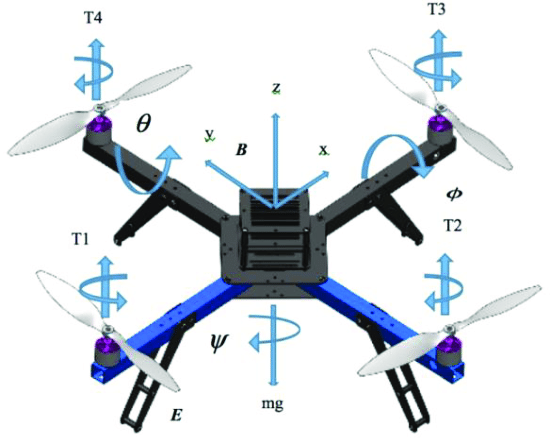
\includegraphics[width=6cm, height=5.5cm]{fuerzas_drone}
    \caption[Caption for LOF]{Cuadric\'{o}ptero\protect\footnotemark}
  \end{figure}
  \footnotetext{Designing and Modeling of Quadcopter Control System Using L1 Adaptive Control Thu et al. 2017}
\end{frame}

\begin{frame}{Control de cuadric\'{o}ptero}
  Control independiente (desacoplado) de la altura, el avance, desplazamiento lateral y el cabeceo por medio de una combinaci\'{o}n intuitiva de la velocidad de giro de los rotores %(CITAR controles 2011)

  \begin{figure}
    \centering
    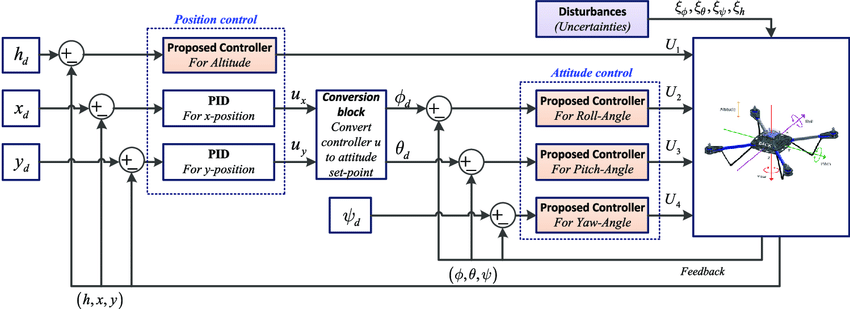
\includegraphics[width=9.5cm, height=4.5cm]{control_drone}
    \caption[Caption for LOF]{Control PID Cuadric\'{o}ptero\protect\footnotemark}
  \end{figure}
  \footnotetext{Quadcopter Robust Adaptive Second Order Sliding Mode Control Based on PID Sliding Surface Thanh et al. 2018}
  
\end{frame}

%\begin{frame}{}
%  Lograr que un multic\'{o}ptero mantenga una posici\'{o}n estable no es una tarea f\'{a}cil y% se han propuesto diversas t\'{e}cnicas (CITAR control difuso, MPC, programacionn genetica..)
%\end{frame}

%\begin{frame}{}
%  Diversas t\'{e}cnicas buscan proporcionar un sistema de control robusto, pero resultan ser t\'{e}cnicas con alto costo computacional, y los VANTS que vemos, los fabricantes hacen uso de controles ya conocidos como PID. Por la complejidad de estabilizar un VANT en el aire, se se aprovecha el desacople para realizar un control en cascada para encontrar la secuencia a aplicar al VANT 
%\end{frame}

\begin{frame}{Arquitectura de control}
  Las estructuras de \textbf{control reactivas} permiten, a tr\'{a}ves de relaciones simples de tipo \textbf{est\'{i}mulo-respuesta} conocidas como \textit{comportamientos.}\\

  De esta forma se logra separar los problemas del robot en sub-problemas (alta modularidad). permitiendo respuestas r\'{a}pidas y robustas a los cambios que puedan efectuarse en el medio ambiente. Todo esto sin un modelo en memoria de su entorno.\\
  
  Con este tipo de control no es posible garantizar que el robot sea capaz de encontrar una soluci\'{o}n a un problema. Al no tener memoria no es posible resolver problemas que consideren estados pasados del robot.\\
    
\end{frame}

\begin{frame}{}
  La \textbf{arquitectura hibrida} reemplaza la planificaci\'{o}n reactiva, por una ejecuci\'{o}n reactiva. En lugar de tener secuencias, se emplean representaciones en memoria para elaborar un plan previo y s\'{o}lo se vigila en tiempo real la correcta activaci\'{o}n y ejecuci\'{o}n de comportamientos.
  \begin{figure}
    \centering
    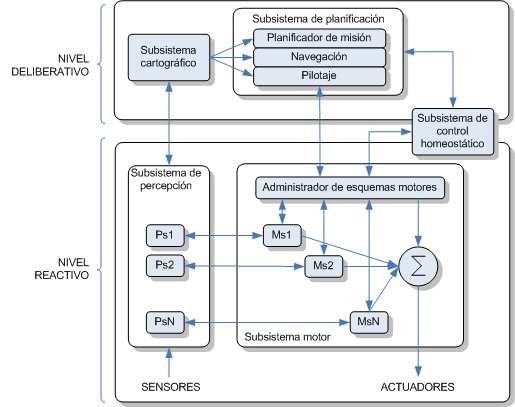
\includegraphics[width=9.5cm, height=4.5cm]{arquitectura_robot.jpg}
    \caption[Caption for LOF]{Arquitectura de control AuRA\protect\footnotemark}
  \end{figure}
  \footnotetext{Revisi\'{o}n de las arquitecturas de control distribuido Posadas et al. 2011}
\end{frame}

\begin{frame}{}
  Tres m\'{o}dulos o capas de control son propuestos para el problema de autonom\'{i}a.
  \bigskip % Vertical whitespace
  \begin{itemize}
  \item Un Planificador - Elabora un plan de ejecuci\'{o}n para alcanzar el objetivo deseado
  \item Habilidades reactivas - Para resolver situaciones precisas
  \item Secuenciador - que conecta las dos anteriores
  \end{itemize}
\end{frame}

\begin{frame}{Planificaci\'{o}n de trayectorias}
  Es un proceso de alto nivel que consume un gran tiempo de c\'{o}mputo. Generalmente no se hace en un tiempo real, apesar que no existe un l\'{i}mite para la complejidad de la soluci\'{o}n, se emplean lenguajes de alto nivel en esta parte.\\

  \begin{figure}
    \centering
    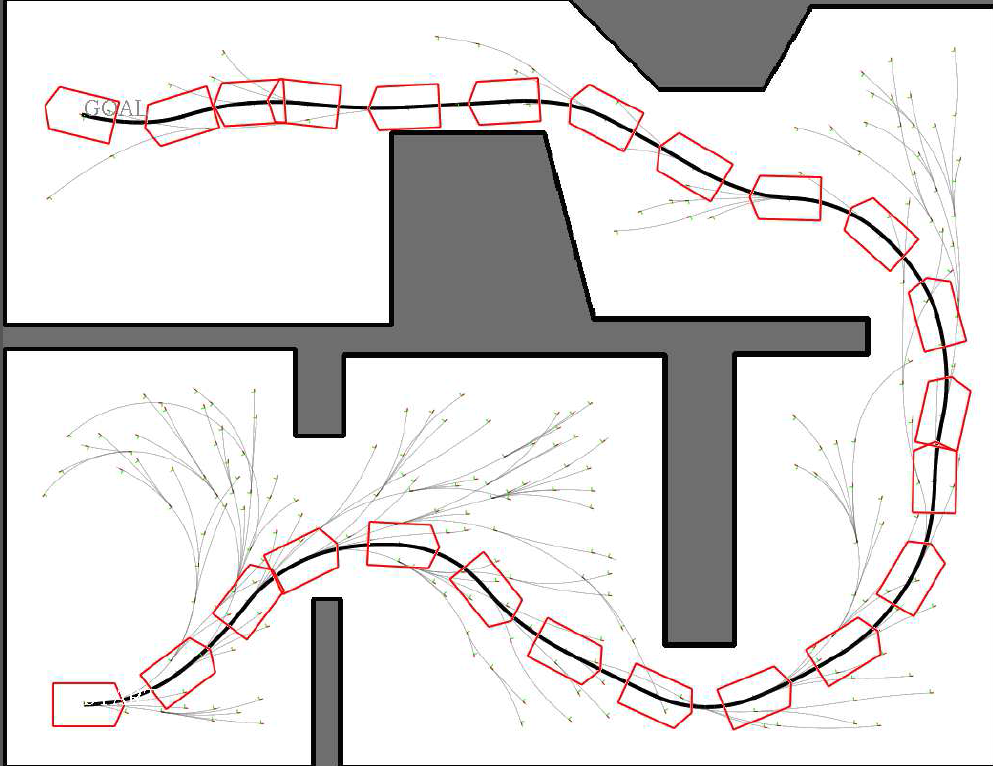
\includegraphics[width=9.5cm, height=4.5cm]{rrt}
    \caption[Caption for LOF]{Algoritmo RRT\protect\footnotemark}
  \end{figure}
  \footnotetext{Randomized kinodynamic planning. LaValle et al. 2001}
  
\end{frame}

\begin{frame}{Controles Primitivos}
  Los controles de bajo nivel son un conjunto de funciones entre el estimulo recogido por los sensores y las acciones efectuadas por el robot. Siendo este un comportamiento o habilidad del robot.\\
  \begin{figure}
    \centering
    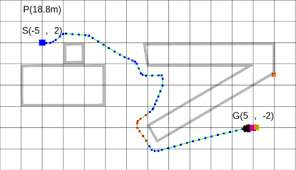
\includegraphics[width=6cm, height=3cm]{bug_algo}
    \caption[Caption for LOF]{Algoritmo Bug\protect\footnotemark}
  \end{figure}
  \footnotetext{Navegación de robots móviles utilizando algoritmos bug. Serna et al. 2019}
  Permiten resolver problemas como evadir obst\'{a}culos. Aqu\'{i} se buscan soluciones y algoritmos en tiempo real.
\end{frame}

\begin{frame}{Secuenciador}
  
  \begin{itemize}
    \item Tiene acceso a la memoria, este recibe el plan desarrollado por la capa deliberativa (Planificador) y selecciona el comportamiento estableciendo los par\'{a}metros m\'{a}s adecuados deacuerdo a su contexto.
    \item Podemos encontrar programas ejecutandose en paralelo, hace uso de interrupciones para tratar situaciones que no se puedan resolver con el programa principal.
  \end{itemize}
      
\end{frame}

\begin{frame}{}
  De esta forma, los tres m\'{o}dulos o capas de control son propuestos para el problema de autonom\'{i}a.
  \begin{itemize}
  \item Un Planificador - Elabora un plan de ejecuci\'{o}n para alcanzar el objetivo deseado
  \item Habilidades reactivas - Para resolver situaciones precisas
  \item Secuenciador - que conecta las dos anteriores
  \end{itemize}
  \begin{figure}
    \centering
    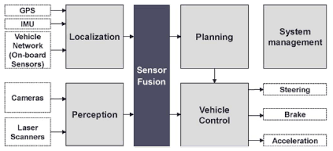
\includegraphics[width=7cm, height=4cm]{control_autonomo}
    \caption[Caption for LOF]{Control Aut\'{o}nomo\protect\footnotemark}
  \end{figure}
  \footnotetext{Software System of Autonomous Vehicles. Guo et al. 2020}
\end{frame}

\begin{frame}{Sistema Aut\'{o}nomo}
  
  \begin{figure}
    \centering
    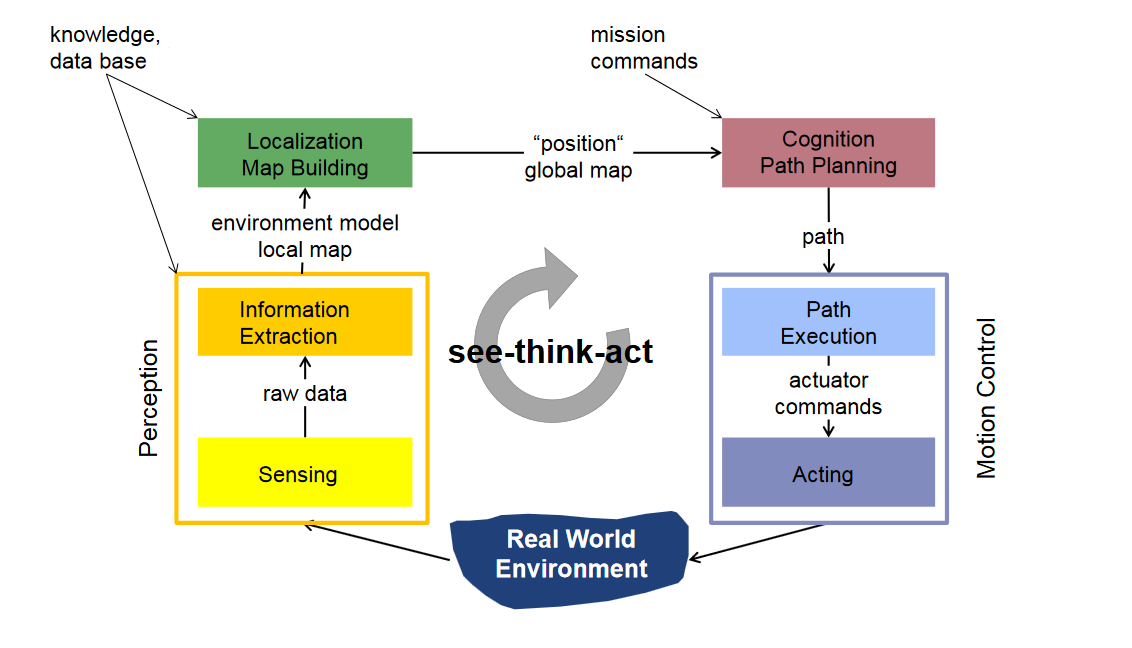
\includegraphics[width=\textwidth, height=5.5cm]{sensar_planear_actuar}
    \caption[Caption for LOF]{Control para un robot m\'{o}vil\protect\footnotemark}
  \end{figure}
  \footnotetext{Siegwart et al., 2011}
\end{frame}

\begin{frame}{¿Qu\'{e} es Planificar?}
  \setlength{\leftmargini}{0.5em}
  \begin{columns}[c, onlytextwidth]%EVEN SPECIFYING THE c OPTION
    \begin{column}{.5\textwidth}%
      \setlength{\partopsep}{0pt}%AND EVEN REMOVING EXTRA itemize SPACE
      \begin{itemize}
        \itemsep 1.5em
      \item <1-> Encontrar una secuencia valida de configuraciones para mover un robot del punto A al punto B; pero .. ¿C\'{o}mo?
      \item <2-> Dados:
        \begin{itemize}
        \item Configuracion inicial A
        \item Configuracion objetivo B
        \item Modelo del robot
        \item Mapa del ambiente
        \end{itemize}
      \end{itemize}
    \end{column}%
    \begin{column}{.45\textwidth}
      \begin{center}
        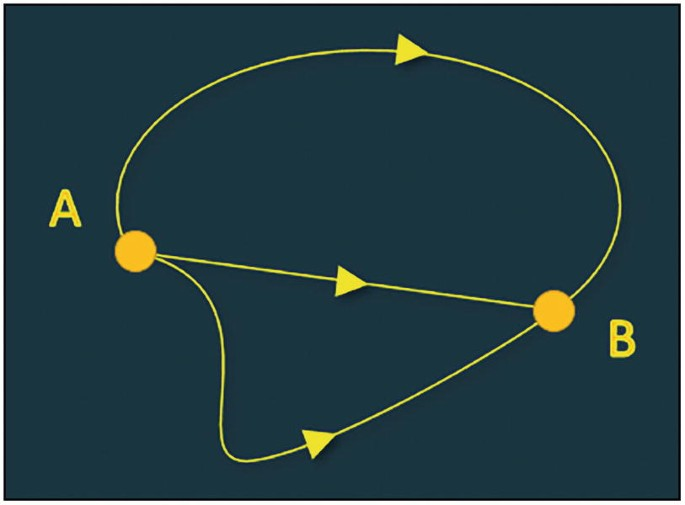
\includegraphics[width=\textwidth, height=5.5cm]{path}
      \end{center}
    \end{column}%
\end{columns}
\end{frame}

\begin{frame}{Planificaci\'{o}n Global vs. Local}
  \begin{figure}
    \centering
    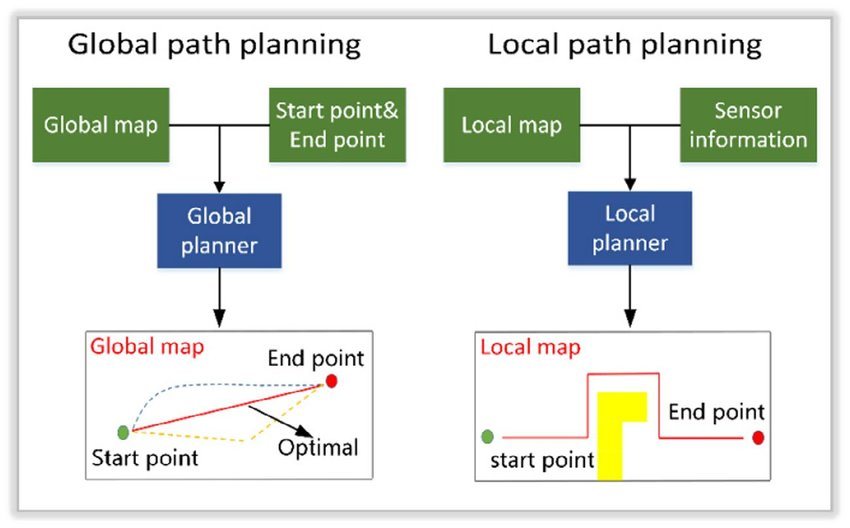
\includegraphics[width=\textwidth, height=5.5cm]{global_local}
    \caption[Caption for LOF]{Planificación Gobal, Planificación Local\protect\footnotemark}
    \footnotetext{A survey on vision-based UAV navigation Zhang 2018}
  \end{figure}
\end{frame}

%\begin{frame}{Configuraci\'{o}nes}
%  \begin{itemize}
%  \item <1-> Configuracion q: especifica todos los puntos del robot respecto a las coordenadas del sistema
%  \item <2-> Ejemplos:\\
%    \centering
%    
\includegraphics[angle=45,width=4cm]{cinvestavlogo}
%    
\includegraphics[angle=45,width=4cm]{cinvestavlogo}
%  \end{itemize}
%\end{frame}

%\begin{frame}{Espacio de Configuraci\'{o}nes}
%  \begin{itemize}
%  \item <1-> Espacio de Configuracion (C-space): espacio de todas las posibles configuraciones
%  \item <2-> Workspace: conjunto de puntos que el robot puede alcanzar.
%  \item Ejemplos\\
%    \centering
%    
\includegraphics[angle=45,width=4cm]{cinvestavlogo}
%    
\includegraphics[angle=45,width=4cm]{cinvestavlogo}
%  \end{itemize}
%\end{frame}

\begin{frame}
  \frametitle{Espacio de Configuraci\'{o}n}
  \setlength{\leftmargini}{0.5em}
  \begin{columns}[c, onlytextwidth]%EVEN SPECIFYING THE c OPTION
    \begin{column}{.5\textwidth}%
      \setlength{\partopsep}{0pt}%AND EVEN REMOVING EXTRA itemize SPACE
      \begin{itemize}
        \itemsep 1.5em
      \item Espacio Libre $C_{free}$ y Espacio Ocupado $C_{obs}$
        El espacio de configuraciones será encontrar un conjunto de puntos de estado del robot $q_{1},...,q_{k}$\\
      \end{itemize}
    \end{column}%
    \begin{column}{.45\textwidth}
      \begin{center}
        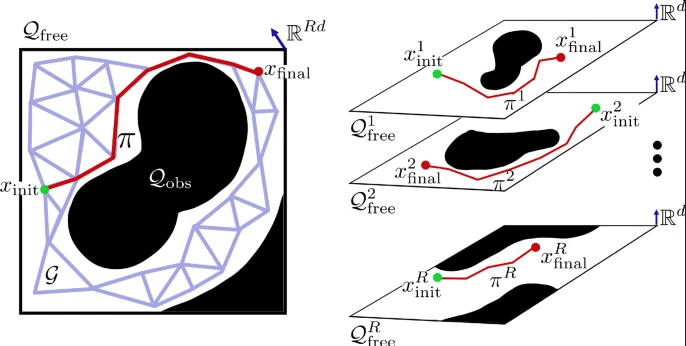
\includegraphics[width=\textwidth, height=5cm]{path2}
      \end{center}
    \end{column}%
\end{columns}
\end{frame}

\begin{frame}{Problema de Planificación}
  \begin{itemize}
  \item Dada una configuración inicial $q_{s}$ y una configuración objetivo $q_{g}$, encontrar un camino continuo que sastiface $\tau (0) = q_{s}, \tau (1)=q_{g}$, y $\tau :[0,1] \rightarrow C_{free}$ \\
    \centering
    \bigskip % Vertical whitespace
    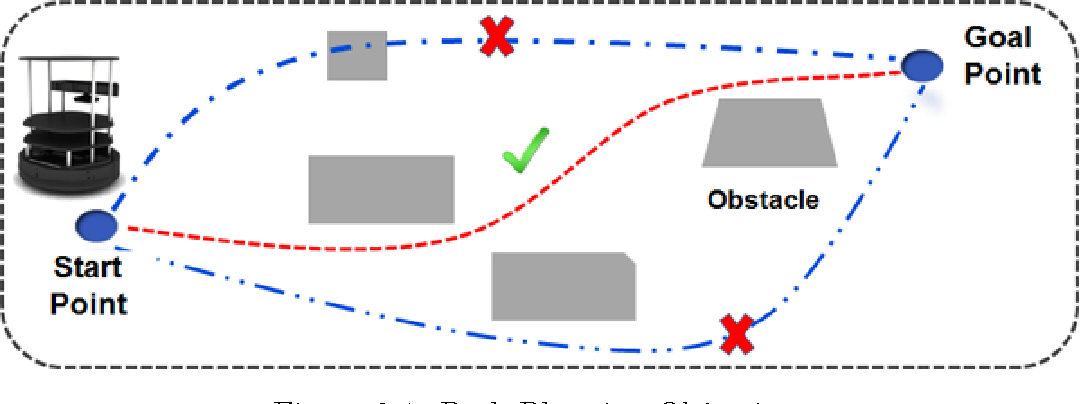
\includegraphics[angle=0,width=8cm]{path_plan}
  \end{itemize}
\end{frame}

%\begin{frame}{Consideraciones}
%  \centering
%  \fbox{\parbox[t]{10em}{
%      \begin{itemize}
%        \tiny \item Caracteristicas Robot
%        \begin{itemize}
%        \tiny \item Grados de libertad
%        \tiny \item Fisica del robot
%        \tiny \item limitaciones en Mobilidad
%        \tiny\item limitaciones en Dinamica
%        \end{itemize}
%      \end{itemize}
%    }
%  }%
%  \raisebox{-4ex}{$\to$}%
%  \fbox{\parbox[t]{10em}{
%      \begin{itemize}
%      \tiny \item Propiedades del algortimo
%        \begin{itemize}
%        \tiny \item Optimalidad
%        \tiny \item Costo Computacional
%        \tiny \item Costo en memoria
%        \tiny \item Completez
%        \tiny \item Online vs. Offline
%        \tiny \item Anytime
%        \tiny \item Caminos vs. trayectorias
%        \tiny \item Exactos vs. aproximados
%%        
%        \end{itemize}
%      \end{itemize}
%    }
%  }
%  \obeylines\\
%\end{frame}

\begin{frame}{Panorama de m\'{e}todos de planificaci\'{o}n}
  \begin{itemize}
  \item Geom\'{e}tricos
    \begin{itemize}
    \item Grafos de visibilidad, descomposici\'{o}n en celdas, diagramas de voronoi, etc.
    \end{itemize}
  \item Campos de potencial
    \begin{itemize}
    \item Frentes de onta, funciones de navegaci\'{o}n, etc.
    \end{itemize}
  \item Basados en b\'{u}squeda
    \begin{itemize}
    \item Dijkstra, A*, D*, D* Lite, etc.
    \end{itemize}
  \item Basados en pruebas
    \begin{itemize}
    \item RRT, RRT*, PRM, etc.
    \end{itemize}
  \item Trayectorias
    \begin{itemize}
    \item M\'{i}nimo tiempo/energia, etc.
    \end{itemize}
  \item Bioinspirados
    \begin{itemize}
    \item Redes Neuronales, Algoritmos Geneticos, Ant Colony Optimisation, etc.
    \end{itemize}
  \end{itemize}
\end{frame}

\begin{frame}{Metodos Geometicos}
  \begin{itemize}
  \item Mapa de ruta con la informacion de la conectividad de los espacios libres\\
    \begin{itemize}
    \item Vertice
    \item Arista
    \end{itemize}
  \item Planes usando algoritmos de grafos\\
    \bigskip % Vertical whitespace
    \begin{figure}
      \centering
      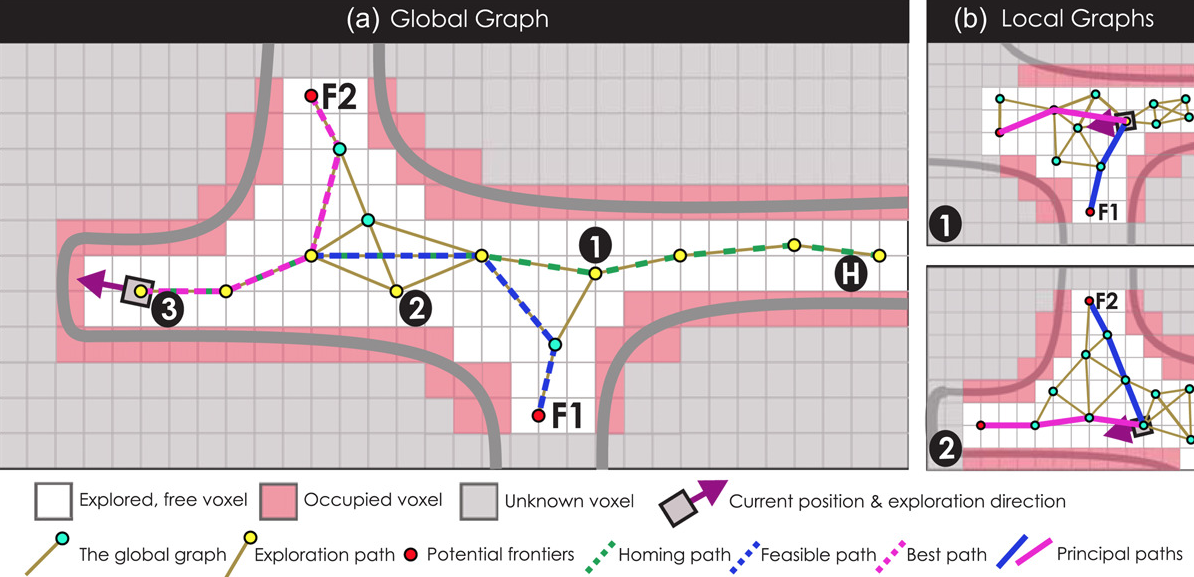
\includegraphics[angle=0,width=8cm]{path_graph}
      \caption[Caption for LOF]{Global exploration planning layer\protect\footnotemark}
      \footnotetext{Graph-based subterranean exploration path planning using aerial and legged robots Tranzatto et al. 2020}
    \end{figure}
  \end{itemize}
\end{frame}

\begin{frame}{Metodos Geometicos}
  \begin{itemize}
  \item Grafo de visibilidad\\
  \item Idea: Conectar todos los vertices visibles  de los obstaculos\\
  \item Planear un camino desde el inicio al objetivo atravez de las aristas: Conectar todos los vertices visibles  de los obstaculos\\
  \item Camino mas corto para obstaculos poligonales\\
  \item Limitantes: Muy cerca de los obstaculos\\
    \centering
    \bigskip % Vertical whitespace
    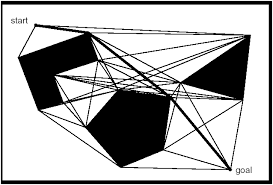
\includegraphics[width=6cm]{visibilidad}
  \end{itemize}
\end{frame}

\begin{frame}{Metodos Geometicos}
  \begin{itemize}
  \item Diagramas de voronoi\\
  \item Idea: Conectar todos los vertices visibles  de los obstaculos\\
  \item Planea una ruta\\
    \centering
    \bigskip % Vertical whitespace
    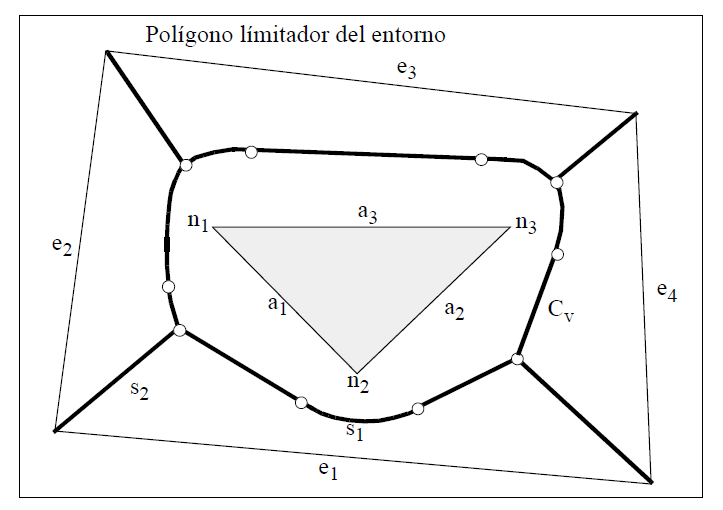
\includegraphics[width=6cm]{voronoi}
  \end{itemize}
\end{frame}

\begin{frame}{Metodos Geometicos}
  \begin{itemize}
  \item Diagrama de voronoi\\
  \item Beneficios\\
    \begin{itemize}
    \item Rutas conservadoras
    \item Similar al comportamiento humano
    \end{itemize}
  \item Limitaciones\\
    \begin{itemize}
    \item Dificil de calcular para altas dimencionalidades
    \item Inestable - cambios minimos en el entorno el diagrama cambia completamente
    \end{itemize}    
    \centering
    \bigskip % Vertical whitespace
    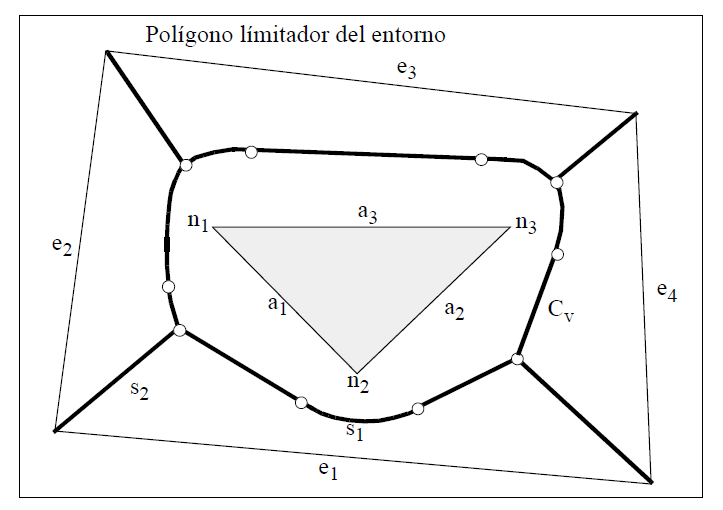
\includegraphics[width=6cm]{voronoi}
  \end{itemize}
\end{frame}

\begin{frame}{Metodos Campo de potencial}
  \begin{itemize}
  \item El Robot es una masa redonda en un plano inclinado \\
  \item Los campos de potencial artificial son funciones derivables\\
    %$U: R^{m} \implies R$
  \item Potencial de atracción\\
  \item Potencial de repulsión\\
    \centering
    \bigskip % Vertical whitespace
    %$A*B=C$\\
    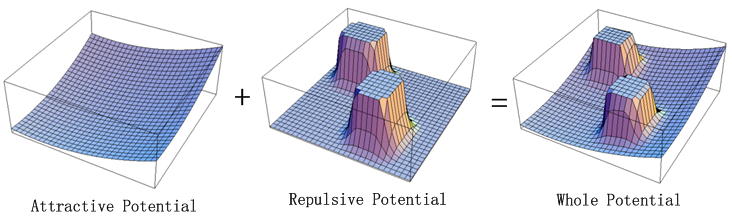
\includegraphics[width=8cm]{potential-field1_robot.jpg}
  \end{itemize}
\end{frame}

\begin{frame}{Metodos Campo de potencial}
  \begin{itemize}
  \item Consideraciones\\
    \begin{itemize}
    \item Modelo del potencial
    \item Solucion del metodo
    \end{itemize}
  \item Idea: seguir el gradiente negativo con uso de desenso de gradiente\\
    \centering
    $F(q)=-\Delta U(q)$\\
    \bigskip % Vertical whitespace
    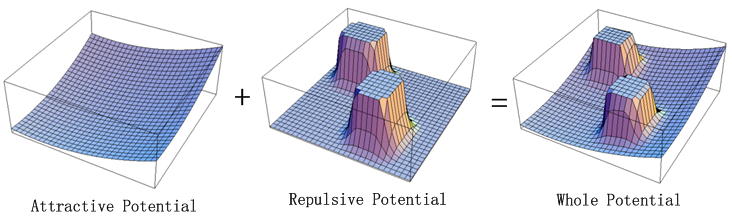
\includegraphics[width=8cm]{potential-field1_robot.jpg}
  \end{itemize}
\end{frame}

\begin{frame}{Metodos Campo de potencial}
  \begin{itemize}
  \item Beneficios\\
    \begin{itemize}
    \item Implementacion sencilla
    \item Evacion de obstaculos online
    \end{itemize}
  \item Limitaciones\\
    \begin{itemize}
    \item Escalabilidad
    \item Minimo local
    \end{itemize}
    %\centering
    %
\includegraphics[angle=45,width=4cm]{cinvestavlogo}
    %
\includegraphics[angle=45,width=4cm]{cinvestavlogo}
  \end{itemize}
\end{frame}

\begin{frame}{Metodos basados en busquedas}
  \begin{itemize}
  \item Planificacion a partir de un grafo $G=(V,E)$\\
    \begin{itemize}
    \item $V$ es un conjunto de vertices $\rightarrow$ configuraciones
    \item $E$ es un conjunto de aristas $\rightarrow$ conecciones libres de colisiones
    \end{itemize}
  \item Aplicar algoritmos de busqueda para encontrar un camino\\
    \begin{itemize}
    \item DFS,BFS,Dijkstra, $A*$, etc.
    \end{itemize}
  \item Ejemplo: Grafo de visibilidad $+$ Dijkstra\\
    \centering
    \bigskip % Vertical whitespace
    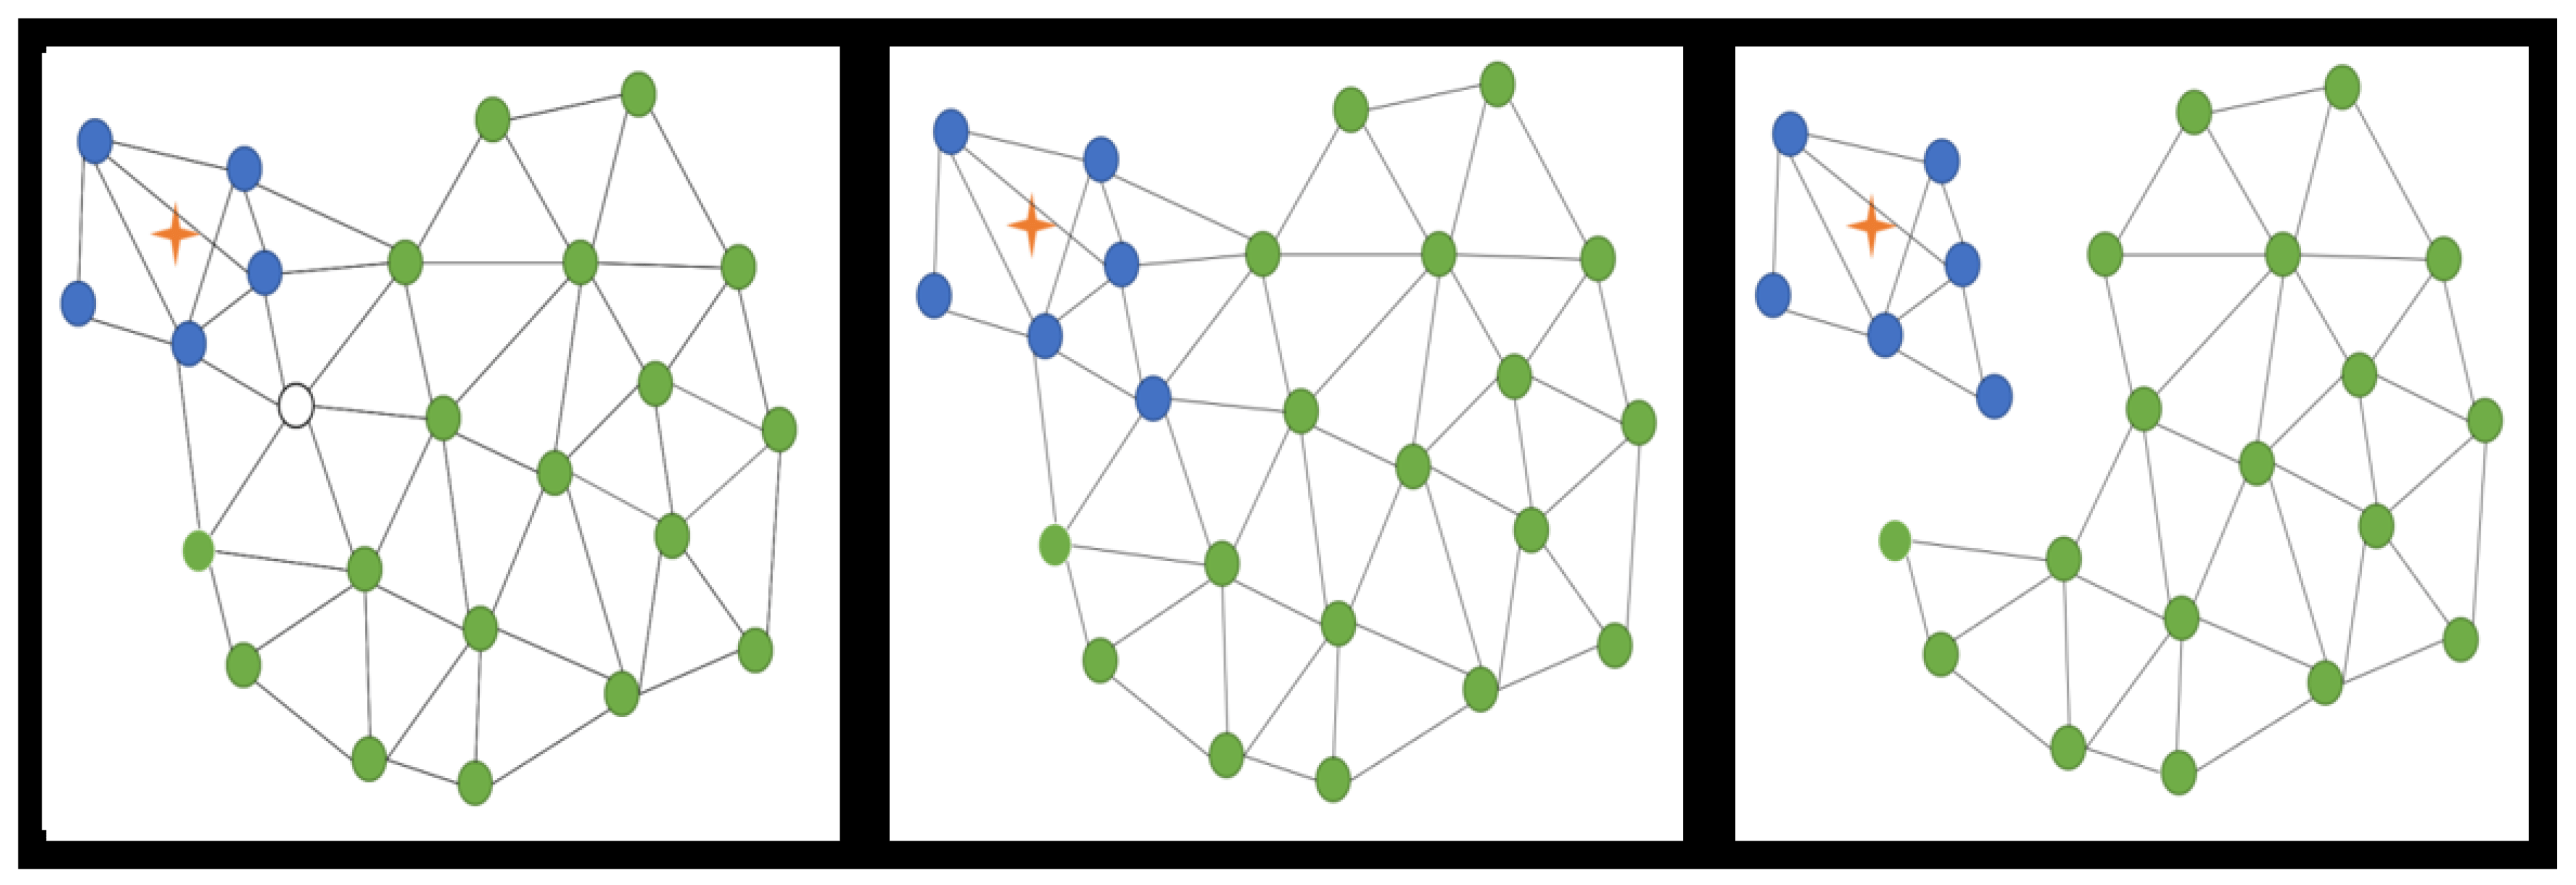
\includegraphics[width=7cm]{graph_robot}
  \end{itemize}
\end{frame}

\begin{frame}{Metodos basados en busquedas}
  \begin{itemize}
  \item Mapa por celdas (Caso especial de un grafo)\\
  \item Se subdivide el $C_{free}$ en pequeñas celdas\\
  \item Permite planificaciones con metodos discretos\\
    \centering
    \bigskip % Vertical whitespace
    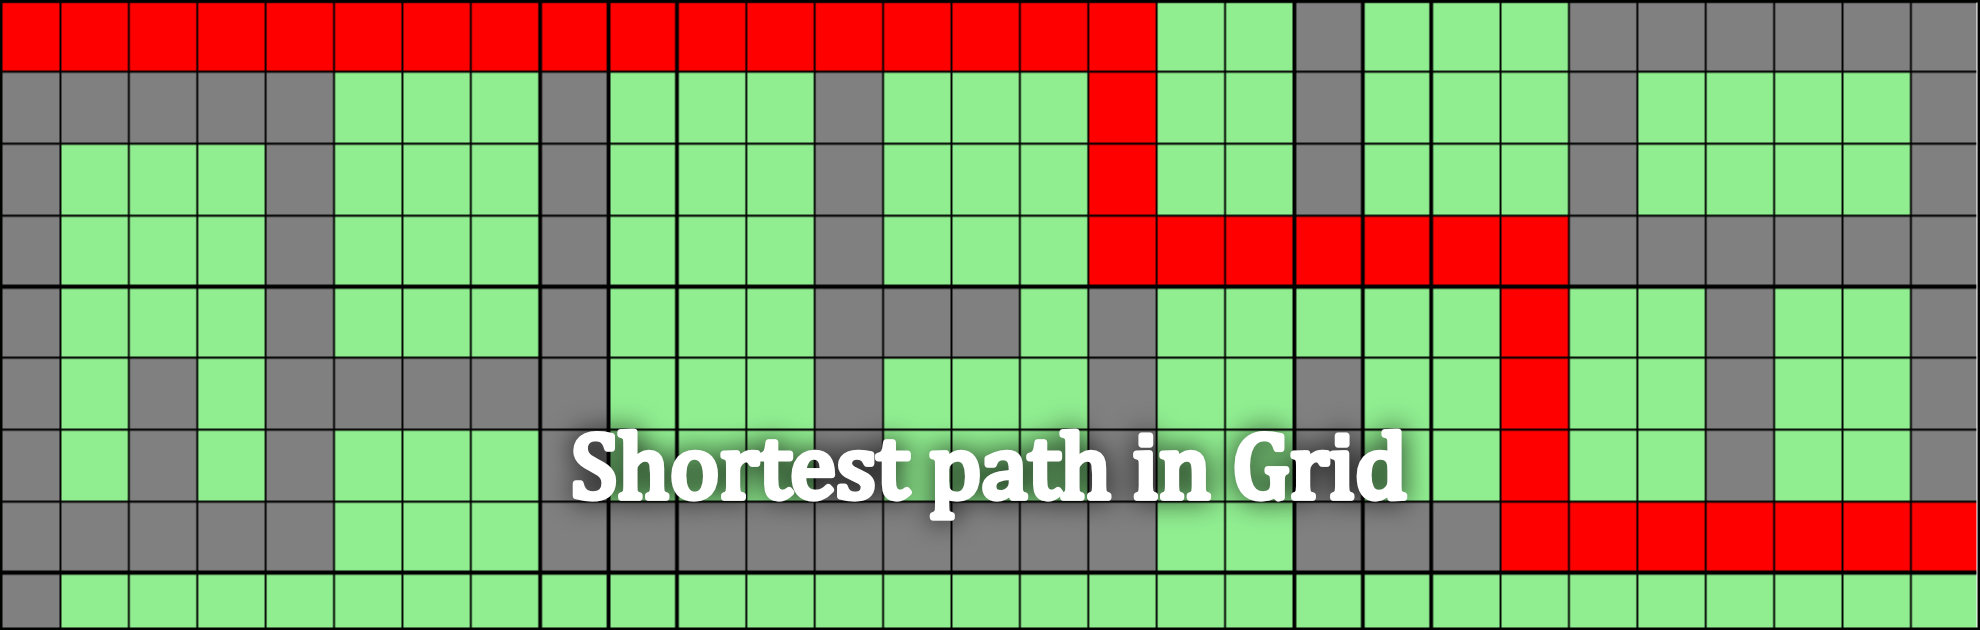
\includegraphics[width=8cm]{bfs.jpg}
  \end{itemize}
\end{frame}

\begin{frame}{Metodos basados en busquedas}
  \begin{itemize}
  \item Ejemplo: Algoritmo de \textbf{Dijkstra} Expande los nodos con una distancia minima al nodo de origen\\
    \centering
    
\includegraphics[angle=45,width=4cm]{cinvestavlogo}
  \end{itemize}
\end{frame}

\begin{frame}{Metodos basados en busquedas}
  \begin{itemize}
  \item Ejemplo: Algoritmo \textbf{A$*$} Considera una heuristica basada en la distancia al objetivo\\
    \centering
    
\includegraphics[angle=45,width=4cm]{cinvestavlogo}
  \end{itemize}
\end{frame}

\begin{frame}{Metodos a partir de pruebas}
  \begin{itemize}
  \item Ejemplo: Probabilistic roadmap (PRM)\\
    \centering
    fase de aprendizaje\\
    
\includegraphics[angle=45,width=4cm]{cinvestavlogo}
    fase de busquedas\\
    
\includegraphics[angle=45,width=4cm]{cinvestavlogo}
  \end{itemize}
\end{frame}

\begin{frame}{Metodos a partir de pruebas}
  \begin{itemize}
  \item Ejemplo: Rapidly-exploring random tree (RRT)\\
    \centering
    
\includegraphics[angle=45,width=4cm]{cinvestavlogo}
  \end{itemize}
\end{frame}

\begin{frame}{}
  \centering
  \begin{tabular}{ |p{1cm}||p{0.8cm}|p{0.8cm}|p{1.2cm}|p{5cm}|  }
    \hline
    \multicolumn{5}{|c|}{\tiny Comparaci\'{o}n de m\'{e}todos} \\
    \hline 
    \tiny Metodo& \tiny Completo & \tiny Optimo& \tiny Escalable& \tiny Notas \\
    \hline
    \tiny Visibility   & \tiny Si    & \tiny Si&   \tiny No& \tiny Poca escalabilidad, el robot pasa cerca de los obstaculos\\
    \hline
    \tiny Voronoi   & \tiny Si    & \tiny No&   \tiny No& \tiny Poca escalabilidad\\
    \hline
    \tiny Potential field   & \tiny Si    & \tiny No&   \tiny Depende del ambiente& \tiny Facil de implementar, suceptible a minimos locales\\
    \hline
    \tiny Dijkstra/A*   & \tiny Si    & \tiny Grid&   \tiny No& \tiny A* usa una funcion heuristica que guia la busqueda mas eficiente, Poca escalabilidad\\
    \hline
    \tiny PRM   & \tiny Si    & \tiny Grafo&   \tiny Si&  \tiny Eficiente para multi-busquedas, completez probabilistica \\
    \hline
    \tiny RRT   & \tiny Si    & \tiny No&   \tiny Si&  \tiny Eficiente para problemas simples, completez probabilistica\\
    \hline
  \end{tabular}  
\end{frame}

\begin{frame}{Sistemas Multi-Robot}
  \FourQuad%
   { \begin{itemize}
      \item<1-> Dado un conjunto de robots que pueden cooperar y comunicarse entre si para realizar ciertas tareas\\
     \end{itemize}\vspace{2cm}\hspace{2.7cm}
   }
   {
     
\includegraphics[width=0.5\textwidth]{cinvestavlogo}
   }
   {
     
\includegraphics[width=0.5\textwidth]{cinvestavlogo}
   }
   {
     
\includegraphics[width=0.5\textwidth]{cinvestavlogo}
   }

\end{frame}

\begin{frame}{Un solo robot vs. Multi-Robot}
  \begin{columns}
    \column{0.5\textwidth}
    \begin{itemize}
    \item Ventajas
      \begin{itemize}
      \item Mejor
      \item Mejor
      \item Mejor
      \item Mejor
      \end{itemize}
    \end{itemize}
    \column{0.5\textwidth}
    \begin{itemize}
    \item Desventajas
      \begin{itemize}
      \item Mejor
      \item Mejor
      \item Mejor
      \item Mejor
      \end{itemize}
    \end{itemize}
  \end{columns}
\end{frame}

\begin{frame}{Taxonomia Multi-Robot}
  \FourQuad%
      { \begin{itemize}
        \item Comportamiento colectivo
        \end{itemize}\vspace{2cm}\hspace{2.7cm}
      }
      {
        \begin{itemize}
        \item Comunicacion
        \end{itemize}\vspace{2cm}\hspace{2.7cm}
        
      }
      {
        \begin{itemize}
        \item Tomar desiciones
        \end{itemize}\vspace{2cm}\hspace{2.7cm}
        
      }
      {
        \begin{itemize}
        \item Formulacion del problema
        \end{itemize}\vspace{2cm}\hspace{2.7cm}
      }

\end{frame}

\begin{frame}{Centralizado vs. Descentralizado}
  \begin{itemize}
  \item Centralizado
  \item Descentralizado
  \item Hibrido
  \end{itemize}
\end{frame}

\begin{frame}{Centralizado: Acoplado}
  \begin{itemize}
  \item Plan directly in joint
  \item For K robots: 
  \item Use standard planning methods
  \item Problem space
  \item Computationally
  \end{itemize}
\end{frame}

\begin{frame}{Centralizado: Desacoplado}
  \begin{itemize}
  \item First Plan for each robot
  \item Then
  \item Not complete, not optimal
  \end{itemize}
\end{frame}

\begin{frame}{Desentralizado}
  \begin{itemize}
  \item Information 
  \item Suboptimal
  \item Implicit or explicit
  \item Coordination strategies..
  \end{itemize}
\end{frame}

%Robotic Information Gathering


%\begin{frame}{Subfigures in Beamer}
%  You can see in Figure \ref{fig:images} that I have inserted two images, Figures \ref{fig:nature1} and \ref{fig:nature2}, that I can reference independently.
%  \begin{figure}
%   \centering
%    \begin{subfigure}[t]{0.4\textwidth}
%      
\includegraphics[width=0.5\textwidth]{cinvestavlogo}
%      \caption{Image of the nature V1.}
%      \label{fig:nature1}
%    \end{subfigure}
%    \begin{subfigure}[b]{0.4\textwidth}
%      
\includegraphics[width=\textwidth]{cinvestavlogo}
%      \caption{Image of the nature V2.}
%      \label{fig:nature2}
%    \end{subfigure}
%    \caption{Two images I want to insert.}
%    \label{fig:images}
%  \end{figure}
%  \end{frame}

%\begin{frame}
%  \frametitle{Using Columns}
%  \begin{columns}
%    \column{0.5\textwidth}
%    <text>
%    \column{0.5\textwidth}
%    <text>
%  \end{columns}
%\end{frame}

%\begin{frame}
%  \frametitle{Stuff famous linguists asked}
%  Hola mundo \cite{james} \footcite{james} 
%\end{frame}

%\begin{frame}{First images in beamer}
%\centering
%    
\includegraphics[width=4cm,angle=45]{cinvestavlogo}
%    
\includegraphics[angle=45,width=4cm]{cinvestavlogo}
%\end{frame}

%\begin{frame}
%\frametitle{Using Columns}
%\begin{columns}
%\column{0.5\textwidth}
%<text>
%\column{0.5\textwidth}
%\centering
%
\includegraphics[scale=0.5]{cinvestavlogo}
%\end{columns}
%\end{frame}

%\begin{frame}
%\frametitle{List}
%\begin{itemize}
%\item Point A
%\item Point B
%\begin{itemize}
%\item part 1
%\item part 2
%\end{itemize}
%\item Point C
%\item Point D
%\end{itemize}
%\end{frame}

%\begin{frame}
%  \frametitle{Pictures}
%  Observe Figure \ref{fig:question}: it is the
%first figure I have inserted in beamer.
%\begin{figure}
%  \centering
%  
\includegraphics[scale=0.5]{cinvestavlogo}
%  \caption{lion!!}
%  \label{fig:question}
%\end{figure}
%<text>
%\end{frame}

%\begin{frame}{Figure with other content}
%\begin{columns}
% Column 1
%\begin{column}{0.5\textwidth}
%        Here I can explain in detail what the figure See \citet{james}. represents.
%\end{column}
% Column 2    
%\begin{column}{0.5\textwidth}
%    \begin{figure}
%    \centering
%        
\includegraphics[width=0.7\textwidth]{cinvestavlogo}
%        \caption{A figure that is next to a certain explanation.}
%    \end{figure}
%\end{column}
%\end{columns}
%\end{frame}

\begin{frame}{Factorization Methods}
  
  \begin{columns}[t]
    \begin{column}{.3\textwidth}
      \adjincludegraphics[width=.8\linewidth,valign=t]{example-image}
    \end{column}
    \begin{column}{.7\textwidth}
      \textbf{``The problem of distinguishing prime numbers from composites, and of resolving composite numbers into their prime factors, is one of the most important and useful in all of arithmetic."}
      
      \hfill-- Carl Friedrich Gauss
    \end{column}
  \end{columns}
  \vspace*{10pt}
  
  \begin{itemize}
  \item Pollard's $p-1$ algorithm (1974)
    \vspace*{10pt}
  \item Dixon's Random Squares Algorithm (1981)
    \vspace*{10pt}
  \item Quadratic Sieve (QS): Pomerance (1981)
    \vspace*{10pt}
  \item Williams' $p+1$ method (1982)
  \end{itemize}
\end{frame}

%\begin{frame}
%  \fbox{\parbox[t]{6em}{Title \#1\\Item\\Item\\Item\\Item}}%
%  \raisebox{-4ex}{$\to$}%
%  \fbox{\parbox[t]{6em}{Title \#2\\Item\\Item\\Item\\Item\\Item}}%
%  \raisebox{-4ex}{$\to$}%
%  \fbox{\parbox[t]{6em}{Title \#3\\Item\\Item\\Item}}
%  \obeylines\\
%  Cita 1 \citep{james}\\
%  Cita 2 \citet*{8478368}\\
%  Cita 3 \cite{8478368}\\
%  Cita 4 \citet{8478368}\\
%  Cita 5 \citet[chap.~2]{8478368}\\
%  \citep[chap.~2]{james}\\
%  \citep[see][]{james}\\
%  \citep[see][chap.~2]{james}\\
%  \citep*{james}\\
%  \citet{8478368,james}\\
%  \citealp*{james}
%\end{frame}

\begin{frame}
  \begin{tikzpicture}[
      level 1/.style={sibling distance=40mm},
      edge from parent/.style={->,draw},
      >=latex]
    
    % root of the the initial tree, level 1
    \node[root] {Drawing diagrams}
    % The first level, as children of the initial tree
    child {node[level 2] (c1) {Defining node and arrow styles}}
    child {node[level 2] (c2) {Positioning the nodes}}
    child {node[level 2] (c3) {Drawing arrows between nodes}};
    
    % The second level, relatively positioned nodes
    \begin{scope}[every node/.style={level 3}]
      \node [below of = c1, xshift=15pt] (c11) {Setting shape};
      \node [below of = c11] (c12) {Choosing color};
      \node [below of = c12] (c13) {Adding shading};
      
      \node [below of = c2, xshift=15pt] (c21) {Using a Matrix};
      \node [below of = c21] (c22) {Relatively};
      \node [below of = c22] (c23) {Absolutely};
      \node [below of = c23] (c24) {Using overlays};
      
      \node [below of = c3, xshift=15pt] (c31) {Default arrows};
      \node [below of = c31] (c32) {Arrow library};
      \node [below of = c32] (c33) {Resizing tips};
      \node [below of = c33] (c34) {Shortening};
      \node [below of = c34] (c35) {Bending};
    \end{scope}
    
    % lines from each level 1 node to every one of its "children"
    \foreach \value in {1,2,3}
    \draw[->] (c1.195) |- (c1\value.west);
    
    \foreach \value in {1,...,4}
    \draw[->] (c2.195) |- (c2\value.west);
    
    \foreach \value in {1,...,5}
    \draw[->] (c3.195) |- (c3\value.west);
  \end{tikzpicture}
\end{frame}

\begin{frame}
  
  \begin{block}{Resumen}

    {\footnotesize Las últimas decadas se ha visto una explosión en el interés de los Vehículos Aéreos No Tripulados (VANTs o drones), a la par que se han introducido nuevas tecnologías de comunicaciones y cómputo en la nube. Los avances en comunicación han permeado al control de VANTs logrando crear soluciones en búsqueda y rescate, así como soluciones de entrega en la última milla. La mayoria de estas aplicaciones carecen de ser autónomas. Para lograr la autonomía primero se deben resolver problemas clásicos en robótica móvil (Mapeo, Localización y Navegación).\\
      
    Se ha demostrado que es posible dotar de autonomía a un VANT y la mayoría de las soluciones son en exteriores con una mejor lectura de un sensor GPS. Los drones del mañana deberán navegar en áreas urbanas de la mejor manera posible y tener la habilidad de trabajar en coordinación con múltiples agentes.\\
    
    El enfoque de este trabajo es la creación y propuesta de una arquitectura capaz de coordinar múltiples-VANTs.\\
    }
  \medskip 
  
  \noindent \textbf{Palabras claves:} multi-VANT, coordinación multi-agente, arquitectura multi-VANT, 3D Path finding
  
  \end{block}
  
\end{frame}

\section{Descripción del proyecto}

\begin{frame}
  \frametitle{Descripción del proyecto}

  {\footnotesize
  El proyecto de estrategias para la exploración coordinada múlti-VANT se centra en las ventajas de tener múltiples-VANT(s) trabajando en conjunto para mejorar la eficiencia y cobertura de la exploración proponiendo una arquitectura de software que con ayuda de algoritmos que permitan la coordinación eficiente de múltiples-VANT(s) para llevar a cabo tareas de exploración en entornos desconocidos y cambiantes.}
      
\end{frame}

\begin{frame}

  \frametitle{Antecedentes y motivación para el proyecto}
  {\footnotesize
  Millones de Vehículos Aéreos No Tripulados, o también conocidos como drones, han presentado una adopción masiva en diferentes aplicaciones, desde usos civiles (búsqueda y rescate, monitoreo industrial, vigilancia), hasta aplicaciones militares [1]. La popularidad de los VANTs es atribuida a su movilidad omnidireccional.\\

  La idea de utilizar múltiples robots aéreos en un sistema coordinado se basa en el comportamiento de los enjambres de animales (como las abejas o los pájaros, que trabajan juntos de manera colaborativa para lograr objetivos comunes). Ésta inspiración biológica ha llevado al desarrollo de algoritmos y técnicas para coordinar y controlar múltiples VANTs en diferentes aplicaciones.\\

  El interés en la investigación e inovación de soluciones con Vehículos Aéreos No Tripulados ha crecido exponencialmente en años recientes [2,7,8,9,10].\\
  }
  \bigskip % Vertical whitespace
  {\footnotesize
  En recientes años, dotar a los VANTs de inteligencia para explotar la información recolectada de sensores a bordo ha sido y es un área de estudio en robótica móvil aérea (construcción de mapas)[3]. Así también los VANTs han sido un módelo interesante de estudio en control por ser marginalmente estable. Convirtiéndo los problemas típicos de control 2D (péndulo inverso fijo) a ambientes 3D [4].
  }
  
\end{frame}

\begin{frame}
  Calcular la ruta más corta entre dos puntos en un ambiente 3D es un problema NP-hard[21]. La mayoria de planificadores de rutas hacen uso de heuristicas y metaheuristicas para generar el óptimo más cercano \\
  \bigskip % Vertical whitespace
  Beneficios coordinación múlti-VANT
  \begin{itemize}
  \item Eficiencia y cobertura
  \item Redundancia y tolerancia a fallos
  \item Adaptabilidad a entornos dinámicos
  \item Distribución de carga de trabajo
  \item Aprendizaje colaborativo
  \end{itemize}
\end{frame}

\section{Planteamiento del problema}

\begin{frame}
  \frametitle{Planteamiento del problema}
  
  La coordinación múlti-VANT es un desafío complejo y plantea diversas problemáticas que deben abordarse.
  \bigskip % Vertical whitespace
  \begin{itemize}
  \item<1-> Coordinación - Establecer comunicación efectiva entre los múltiples VANTs. Intercambiar información relevante. Tener baja latencia en su comunicación.
  \item<2-> Planificación - Los VANTs deben coordinar sus movimientos para evitar colisiones y lograr una cobertura eficiente del área objetivo.
  \item<3-> Asignación de tareas - Se busca evitar la duplicación de esfuerzos optimizando el uso de recursos disponibles.
  \end{itemize}
  
\end{frame}

\begin{frame}
  Dada un área de interés \textbf{A} desconocido que se desea explorar, un conjunto de VANTs denotados como \textbf{$V=V_{1},V_{2},V_{3},...,V_{n}$}, donde $n$ es el número total de VANTs disponibles, un conjunto de tareas de exploración denotados como \textbf{$T=T_{1},T_{2},T_{3},...,T_{m}$}, donde $m$ es el número total de tareas a realizar.\\
  \bigskip % Vertical whitespace
  Teniendo restricciones y requisitos específicos del problema, como límites de tiempo, obstáculos a evitar ... etc.\\

  Para las tareas de exploración $T_{m}$, se considerán las siguientes variables:

  \begin{itemize}
  \item Posición inicial: $p_{i}(x,y,z)$, posición inical VANTs
  \item Trayectoria: $\alpha_{i}$, trayectoria seguida por los VANTs asignados a la tarea $T_{m}$ en función del tiempo t
  \item Información recolectada: $C_{i}$, representa la información recolectada por los VANTs asignados durante la exploración
  \end{itemize}
  
\end{frame}

\begin{frame}
  La función objetivo puede cambiar, algunos ejemplos pueden ser:
  \bigskip % Vertical whitespace
  \begin{itemize}
  \item Maximizar la cobertura del área de interés \textbf{A}
  \item Minimizar el tiempo total requerido para cubrir el área de interés \textbf{A}
  \item Maximizar la cantidad de información recolectada
  \end{itemize}
  
\end{frame}

\section{Objetivos generales y específicos del proyecto}

\begin{frame}
  
  \frametitle{Objetivos generales y específicos del proyecto}

  \begin{enumerate}
  \item<1-> General \\

    Desarrollo e implementación de una arquitectura de software tolerante a fallas para la coordinación de múltiples VANTs con un enfoque simulado en búsqueda y rescate.
        
  \item<2-> Particulares\\

    \begin{itemize}
    \item<1-> Generación del modelo dinámico de un VANT 
    \item<2-> Creación de algoritmos reactivos de baja memoria que garanticen evitar colisiones
    \item<3-> Eficiencia y rendimiento del sistema
    \item<4-> Adaptabilidad y flexibilidad, la coordinación múlti-VANT debe ser adaptable a cambios en el entorno, nuevos objetivos y adaptable a la incorporación o salida de VANTs durante la exploración
    \end{itemize}
    
  \end{enumerate}
\end{frame}

\section{Metodología}

\begin{frame}

  \frametitle{Metodología}
  \bigskip % Vertical whitespace

  \begin{enumerate}
  \item <1-> Revisión de literatura 
    \begin{itemize}
    \item Realizar una revisión de la literatura científica y técnica relacionada con la coordinación de múltiples VANTs
    \item Identificar los enfoques existentes, algoritmos y tecnologías usadas en la coordinación de múltiples VANTs
    \end{itemize}
  \item <2-> Análisis y diseño de la solución propuesta
    \begin{itemize}
    \item Identificar los requisitos clave para una coordinación eficiente
    \item Propuesta de algoritmos y políticas de navegación que permitan la coordinación eficiente
    \item Estrategias para la repartición de tareas y gestión de recursos.
    \end{itemize}
  \item <3-> Implementación y validación
    \begin{itemize}
    \item Hacer uso de simuladores (Son baratos, rápidos .. pero la solución está lejos de la solución propuesta en el ambiente real).
    \item Evaluar el desempeño de la coordinación
    \end{itemize}
  \item <4-> Evaluación, resultados y conclusiones
    \begin{itemize}
    \item Analizar y comparar los resultados obtenidos con otros enfoques existentes.
    \item Identificar posibles mejoras y áreas de investigación futuras
    \end{itemize}
  \end{enumerate}
  
\end{frame}


\section{Estado del Arte}

\begin{frame}
  \cite{CIESLEWSKI2017}\\
  \cite{USENKO2017}\\
  \cite{MOHTA2017}\\
\end{frame}
\begin{frame}
  \cite{LIN2017}\\
  \cite{PAPACHRISTOS2017}\\
  \cite{OLEYNIKOVA2018}\\
\end{frame}
\begin{frame}
  \cite{GAO2018}\\
  \cite{FLORENCE2018}\\
  \cite{SELIN2019}\\
\end{frame}
\begin{frame}
  \cite{COLLINS2019}\\
  \cite{CINVES2021}\\
  \cite{RACER2022}\\
\end{frame}
\begin{frame}
  \cite{WESTHEIDER2023}\\
  \cite{BARTOLOMEI2023}\\
\end{frame}

\section{Contribuciones o resultados esperados}

\begin{frame}

  \frametitle{Contribuciones o resultados esperados}

  \begin{enumerate}
  \item<1-> Códigos a disposición de la comunidad
  \item<2-> Simulación de solución
  \item<3-> Tesis impresa
  \end{enumerate}
  
\end{frame}

\begin{frame}
  \frametitle{Bibliography}
  \bibliographystyle{abbrvnat}
  \bibliography{test}
\end{frame}

\end{document} 
